\documentclass[12pt]{article}
\usepackage{xeCJK}%preamble part
\usepackage{graphicx}
\usepackage{indentfirst}
\usepackage[a4paper, inner=1.5cm, outer=3cm, top=2cm, bottom=3cm, bindingoffset=1cm]{geometry}
\usepackage{epstopdf}
\usepackage{listings}
\usepackage{array}
\usepackage{fontspec}
\usepackage{gensymb}
\usepackage{todonotes}
\usepackage{amsmath}
\usepackage[citecolor=blue]{hyperref}

\usepackage{makecell}
\usepackage[lofdepth,lotdepth]{subfig}




\setlength{\extrarowheight}{4pt}
\setlength{\parindent}{1cm}
\begin{document}
\title{\textbf{\fontsize{15.75pt}{\baselineskip}{讨论}}} 

\author{\fontsize{12pt}{\baselineskip}{数33 赵丰}}
\maketitle
\large
在Fundamental limits of wideband localization--Part I: A general framework一文中,

\begin{figure}[!ht]
\centering
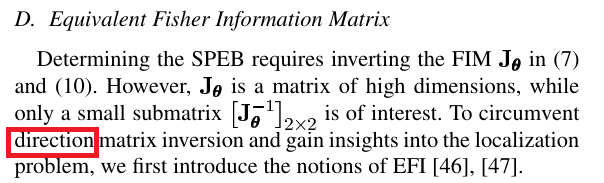
\includegraphics[width=3.0in]{001.png}
\end{figure}

上图direction是否应为direct

如果给定一个连续时间的过程$Y(t),t \to [0,T]$,做检测和估计的方法是首先把$Y(t)$做正交展开,提取系数序列$Z_1,Z_2,...$,通过对有限
序列$Z_1,Z_2,...Z_n$的似然函数取极限得到原问题的似然函数。
一种常见的情形是检测是在高斯噪声模型的情况下检测信号是$s_1(t)$
还是$s_2(t)$,通过取$s_t=s_1(t)-s_2(t)$,问题可以转化为下面的
detection problem:
\begin{equation}
\begin{split}
H_0: Y_t=N_t,0 \leq t \leq T \\
versus\\
H_1:Y_t=N_t+s_t,0 \leq t \leq T 
\end{split}
\end{equation}
$N_t$是理想的高斯白噪声过程,即$N_t \sim N(0,\frac{N_0}{2})$,且任意两个时刻噪声相互独立。通过上面的理论,在已知信号的表达式$s_t$,给定观测值$Y_t$,对数似然比检验是通过如下统计量进行的:
\begin{equation}
\frac{2}{N_0}\int_0^T s_t Y_t dt -\frac{1}{N_0}\int_0^T s_t^2 dt
\end{equation}
记$d^2=\frac{2}{N_0}\int_0^T s_t^2 dt$,
$I_t=\frac{2}{N_0}\int_0^T s_t Y_t dt$
则检验问题实际上是判断$I_t \sim N(0,d^2)$(在$H_0$假定下),还是
$I_t \sim N(d^2,d^2)$(在$H_1$假定下)
上式可以从积分的定义理解,考虑到采样本身是对连续观测样值离散化的过程,而且实际数值计算积分中也是用离散化的方法,因此用
$\sum s_t(iT/n)Y_t(iT/n)T/n$近似$\int_0^T s_t Y_t dt$是有意义的。求和式是若干个独立正态分布的和,故和式仍为正态分布,$Y_t$是否含已知
信号$s_t$对方差没有影响,故有:
\begin{equation}
D(\frac{2}{N_0}\sum_{i=1}^n s_t(iT/n)Y_t(iT/n)T/n)=\frac{4}{N_0^2}\sum_{i=1}^n s_t^2(iT/n)\frac{N_0T^2}{2n^n}
\end{equation}
对$\frac{nD}{T}$取极限$n \rightarrow \infty $即为$d^2$。
另一方面:
\begin{equation}
E(\frac{2}{N_0}\sum_{i=1}^n s_t(iT/n)Y_t(iT/n)T/n)=\frac{2}{N_0} \sum_{i=1}^n \frac{s_t(iT/n)T}{n}E(Y_t(iT/n))
\end{equation}
若$Y_t$只含噪声项,则上式均值为0,若$Y_t=N_t+s_t$,则上式取极限得$d^2$.因此对于连续样值的假设检验问题,可以转化为方差已知情况下
正态总体均值的分类问题,可以用假设检验的一般方法处理。






\end{document}